\documentclass[12pt]{ctexart}
\usepackage[margin=1.8cm]{geometry}
\usepackage{amsmath}
\usepackage{lipsum}
\usepackage{graphicx}
\usepackage{xcolor}
\usepackage{tikz}
\setmainfont{Segoe Print}
\setmonofont{Segoe Script}
\setCJKmainfont{LXGW WenKai}
\usetikzlibrary{calc,intersections} %Task2
\usetikzlibrary{arrows.meta,decorations.pathmorphing,backgrounds,positioning,fit,petri} %Task3
\usetikzlibrary{calc,intersections,through,backgrounds} %Task4
\usetikzlibrary{calc,positioning,shapes.misc} %Task5
\newcounter{taskCounter}
\newcommand{\task}[1]{
  \stepcounter{taskCounter}
  \noindent\textbf{Task\ \arabic{taskCounter} #1} \par
}%
\newcounter{stepCounter}[taskCounter]
\newcommand{\step}[1]{
  \stepcounter{stepCounter}
  \textbf{Step\ \thetaskCounter-\arabic{stepCounter} #1} \par
}
\usepackage{soul}
\definecolor{hlcolour}{rgb}{.75,.75,.75}
\sethlcolor{hlcolour}
\NewDocumentCommand \wordbox { o m }
{%
  \begingroup
    \IfValueT{#1}{\colorlet{hlcolour}{#1}}%如果提供了颜色可选参数则使用该颜色
    \hl{#2}%否则默认使用浅灰色
  \endgroup
}
\pagestyle{empty}
\begin{document}
\task{Try one's hand at TIKZ}
\tikz \draw[thick,rounded corners=8pt] (0,0) -- (0,2) -- (1,3.25) -- (2,2) -- (2,0) -- (0,2) -- (2,2) -- (0,0) -- (2,0);

\task{A Picture for Karl's Students Step by Step}
\scalebox{.55}{
  \includegraphics{./fig/figure1.png}
}

\step{绘制出带箭头的\wordbox{line axis}}
\begin{tikzpicture}
  \draw[-latex] (-1.5,0) -- (1.5,0);
  \draw[-latex] (0,-1.5) -- (0,1.5);
\end{tikzpicture}

\step{绘制\wordbox{help lines}与轮廓}
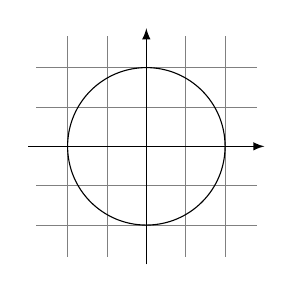
\begin{tikzpicture}
  \draw[step=.5cm,gray,very thin] (-1.4,-1.4) grid (1.4,1.4);
  \draw[-latex] (-1.5,0) -- (1.5,0);
  \draw[-latex] (0,-1.5) -- (0,1.5);
  \draw (0,0) circle [radius=1cm];
\end{tikzpicture}

\step{使用\wordbox{scale}选项并绘制小圆弧和直线}
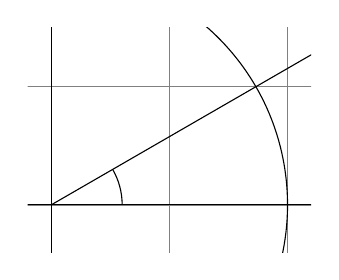
\begin{tikzpicture}[scale=3]
  \clip (-0.1,-0.2) rectangle (1.1,0.75); %剪切只显示局部区域 等价于 \clip[draw]
  \draw[step=.5cm,gray,very thin] (-1.4,-1.4) grid (1.4,1.4);
  \draw[-latex] (-1.5,0) -- (1.5,0);
  \draw[-latex] (0,-1.5) -- (0,1.5);
  \draw (0,0) circle [radius=1cm];
  \draw (3mm,0mm) arc [start angle=0, end angle=30, radius=3mm];
  \draw (0,0) -- ($ (0,0)!1.5cm!30:(1.5,0) $);
  %基于 calc 库调用了 距离-角度定点法进行绘制
\end{tikzpicture}

\step{使用\wordbox{filldraw}命令添加绿色角度标识}
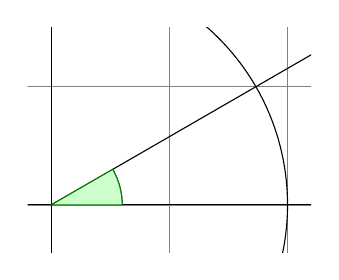
\begin{tikzpicture}[scale=3]
  \clip (-0.1,-0.2) rectangle (1.1,0.75); %剪切只显示局部区域 等价于 \clip[draw]
  \draw[step=.5cm,gray,very thin] (-1.4,-1.4) grid (1.4,1.4);
  \draw[-latex] (-1.5,0) -- (1.5,0);
  \draw[-latex] (0,-1.5) -- (0,1.5);
  \draw (0,0) circle [radius=1cm];
  \draw (3mm,0mm) arc [start angle=0, end angle=30, radius=3mm];
  \draw (0,0) -- ($ (0,0)!1.5cm!30:(1.5,0) $);
  \filldraw[fill=green!20!white, draw=green!50!black] (0,0) -- (3mm,0mm) arc [start angle=0, end angle=30, radius=3mm] -- cycle;
  %基于 calc 库调用了 距离-角度定点法进行绘制
\end{tikzpicture}

\step{添加红色与蓝色坐标定位线}
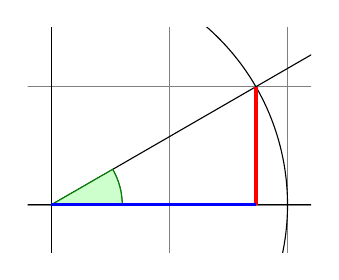
\begin{tikzpicture}[scale=3]
  \clip (-0.1,-0.2) rectangle (1.1,0.75); %剪切只显示局部区域 等价于 \clip[draw]
  \draw[step=.5cm,gray,very thin] (-1.4,-1.4) grid (1.4,1.4);
  \draw[-latex] (-1.5,0) -- (1.5,0);
  \draw[-latex] (0,-1.5) -- (0,1.5);
  \draw (0,0) circle [radius=1cm];
  \draw (3mm,0mm) arc [start angle=0, end angle=30, radius=3mm];
  %基于 calc 库调用了 距离-角度定点法进行绘制
  \draw (0,0) -- ($ (0,0)!1.5cm!30:(1.5,0) $);
  \filldraw[fill=green!20!white, draw=green!50!black] (0,0) -- (3mm,0mm) arc [start angle=0, end angle=30, radius=3mm] -- cycle;
  \draw[red,very thick] (30:1cm) -- +(0,-0.5); %此处手动计算了余弦值,不够优雅
  \draw[blue,very thick] (30:1cm) ++(0,-0.5) -- (0,0); % ++ 修改了当前点
\end{tikzpicture}

\step{小彩蛋:关于\wordbox{+}与\wordbox{++}对当前坐标点的影响}
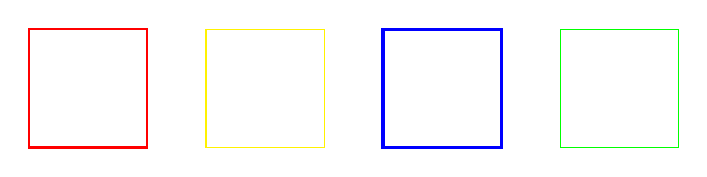
\begin{tikzpicture}[scale=1.5]
  \def\rectanglepathA{-- ++(1cm,0cm) -- ++(0cm,1cm) -- ++(-1cm,0cm) -- cycle}
  \draw[red,thick] (0,0) \rectanglepathA;
  \draw[yellow,thin] (1.5,0) \rectanglepathA;
  \def\rectanglepathB{-- +(1cm,0cm) -- +(1cm, 1cm) -- + (0cm,1cm) -- cycle}
  \draw[blue,very thick] (3,0) \rectanglepathB;
  \draw[green,very thin] (4.5,0) \rectanglepathB;
\end{tikzpicture}

\step{使用路径交点法获取交点并绘制橙色线}
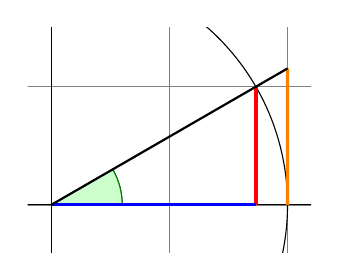
\begin{tikzpicture}[scale=3]
  \clip (-0.1,-0.2) rectangle (1.1,0.75); %剪切只显示局部区域 等价于 \clip[draw]
  \draw[step=.5cm,gray,very thin] (-1.4,-1.4) grid (1.4,1.4);
  \draw[-latex] (-1.5,0) -- (1.5,0);
  \draw[-latex] (0,-1.5) -- (0,1.5);
  \draw (0,0) circle [radius=1cm];
  \draw (3mm,0mm) arc [start angle=0, end angle=30, radius=3mm];
  \filldraw[fill=green!20!white, draw=green!50!black] (0,0) -- (3mm,0mm) arc [start angle=0, end angle=30, radius=3mm] -- cycle;
  \draw[red,very thick] (30:1cm) -- +(0,-0.5); %此处手动计算了余弦值,不够优雅
  \draw[blue,very thick] (30:1cm) ++(0,-0.5) -- (0,0); % ++ 修改了当前的控制点
  \path[name path= upward line] (1,0) -- (1,1);
  \path[name path= sloped line] (0,0) -- (30:1.5cm);
  \draw[name intersections={of = upward line and sloped line,by=x}][very thick, orange] (1,0) -- (x);
  \draw[thick] (0,0) -- (x);
\end{tikzpicture}

\step{使用\wordbox{foreach}命令绘制刻度线}
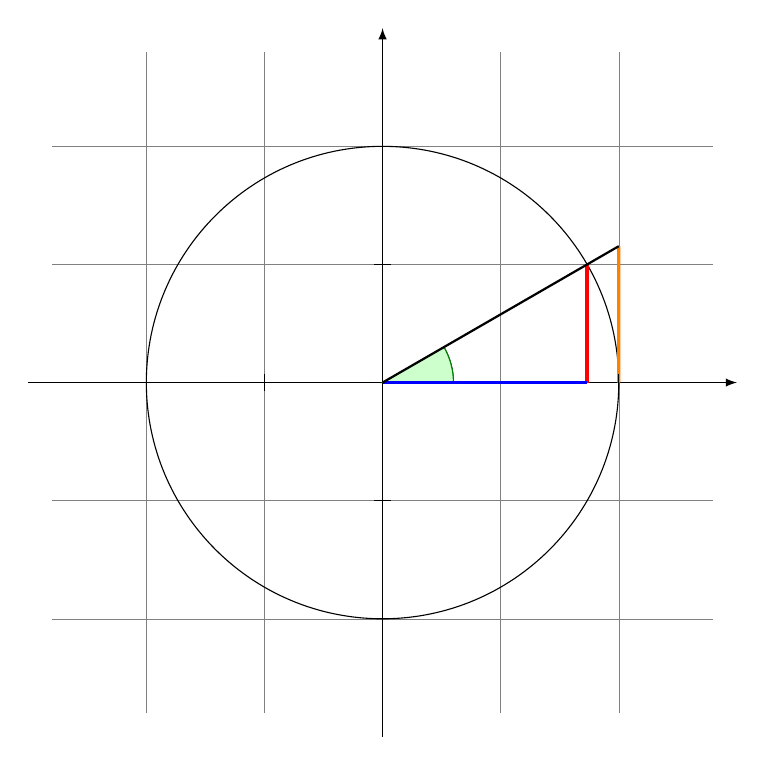
\begin{tikzpicture}[scale=3]
  \draw[step=.5cm,gray,very thin] (-1.4,-1.4) grid (1.4,1.4);
  \draw[-latex] (-1.5,0) -- (1.5,0);
  \draw[-latex] (0,-1.5) -- (0,1.5);
  \draw (0,0) circle [radius=1cm];
  \draw (3mm,0mm) arc [start angle=0, end angle=30, radius=3mm];
  \filldraw[fill=green!20!white, draw=green!50!black] (0,0) -- (3mm,0mm) arc [start angle=0, end angle=30, radius=3mm] -- cycle;
  \draw[red,very thick] (30:1cm) -- +(0,-0.5); %此处手动计算了余弦值,不够优雅
  \draw[blue,very thick] (30:1cm) ++(0,-0.5) -- (0,0); % ++ 修改了当前的控制点
  \path[name path= upward line] (1,0) -- (1,1);
  \path[name path= sloped line] (0,0) -- (30:1.5cm);
  \draw[name intersections={of = upward line and sloped line,by=x}][very thick, orange] (1,0) -- (x);
  \draw[thick] (0,0) -- (x);
  \foreach \x in {-1cm,-0.5cm,1cm}
  \draw (\x,-1pt) -- (\x,1pt);
  \foreach \y in {-1cm,-0.5cm,0.5cm,1cm}
  \draw (-1pt,\y) -- (1pt,\y);
\end{tikzpicture}

\step{使用\wordbox{node}命令指定\wordbox{anchor}选项添加文本}
实际上这里要注意\wordbox{node}绘制坐标的方向、\wordbox{anchor}并采用数学模式下的文本.

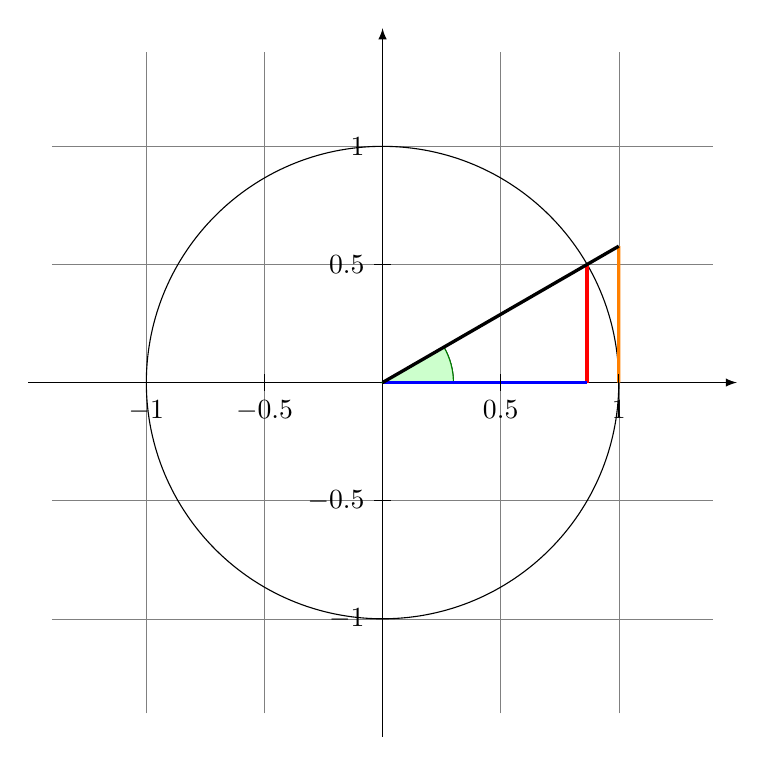
\begin{tikzpicture}[scale=3]
  \draw[step=.5cm,gray,very thin] (-1.4,-1.4) grid (1.4,1.4);
  \draw[-latex] (-1.5,0) -- (1.5,0);
  \draw[-latex] (0,-1.5) -- (0,1.5);
  \draw (0,0) circle [radius=1cm];
  \draw (3mm,0mm) arc [start angle=0, end angle=30, radius=3mm];
  \filldraw[fill=green!20!white, draw=green!50!black] (0,0) -- (3mm,0mm) arc [start angle=0, end angle=30, radius=3mm] -- cycle;
  \draw[red,very thick] (30:1cm) -- +(0,-0.5); %此处手动计算了余弦值,不够优雅
  \draw[blue,very thick] (30:1cm) ++(0,-0.5) -- (0,0); % ++ 修改了当前的控制点
  \path[name path= upward line] (1,0) -- (1,1);
  \path[name path= sloped line] (0,0) -- (30:1.5cm);
  \draw[name intersections={of = upward line and sloped line,by=x}][very thick, orange] (1,0) -- (x);
  \draw[very thick] (0,0) -- (x);
  \foreach \x in {-1,-0.5,0.5,1}
  \draw (\x cm,1pt) -- (\x cm,-1pt) node[anchor=north] {$\x$};
  \foreach \y in {-1,-0.5,0.5,1}
  \draw (1pt,\y cm) -- (-1pt,\y cm) node[anchor=east] {$\y$};
\end{tikzpicture}

\step{添加部分颜色信息标注}
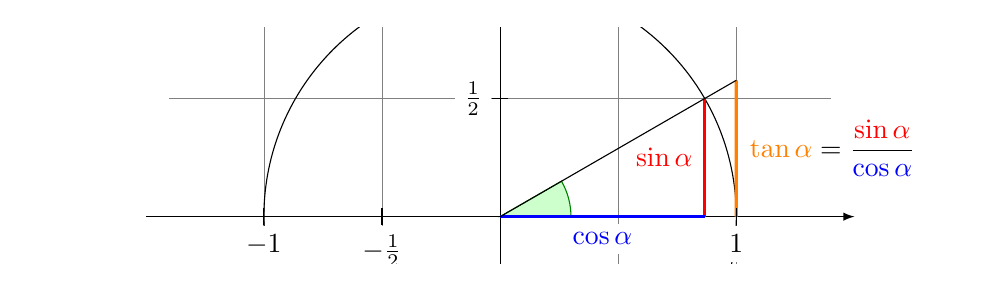
\begin{tikzpicture}[scale=3]
  \clip (-2,-0.2) rectangle (2,0.8);
  \draw[step=.5cm,gray,very thin] (-1.4,-1.4) grid (1.4,1.4);
  \filldraw[fill=green!20,draw=green!50!black] (0,0) -- (3mm,0mm)
  arc [start angle=0, end angle=30, radius=3mm] -- cycle;
  \draw[-latex] (-1.5,0) -- (1.5,0) coordinate (x axis);
  \draw[-latex] (0,-1.5) -- (0,1.5) coordinate (y axis);
  \draw (0,0) circle [radius=1cm];
  \draw[very thick,red]
  (30:1cm) -- node[left=.5pt,fill=white] {$\sin \alpha$} (30:1cm |- x axis);
  %标注\sin的位置为 (30:1cm |- x axis) -- (30:1cm)路径的中点
  \draw[very thick,blue]
  (30:1cm |- x axis) -- node[below=2pt,fill=white] {$\cos \alpha$} (0,0);
  %标注\cos的位置为 (30:1cm |- x axis) -- (0,0)路径的中点
  \path [name path=upward line] (1,0) -- (1,1);
  \path [name path=sloped line] (0,0) -- (30:1.5cm);
  \draw [name intersections={of=upward line and sloped line, by=t}]
  [very thick,orange] (1,0) -- node [right=1pt,fill=white]
  {$\displaystyle \tan \alpha \color{black}=
      \frac{{\color{red}\sin \alpha}}{\color{blue}\cos \alpha}$} (t);
  %标注\tan的位置为 (1,0) -- (t) 路径的中点
  \draw (0,0) -- (t);
  \foreach \x/\xtext in {-1, -0.5/-\frac{1}{2}, 1}
  \draw (\x cm,1pt) -- (\x cm,-1pt) node[anchor=north,fill=white] {$\xtext$};
  \foreach \y/\ytext in {-1, -0.5/-\frac{1}{2}, 0.5/\frac{1}{2}, 1}
  \draw (1pt,\y cm) -- (-1pt,\y cm) node[anchor=east,fill=white] {$\ytext$};
\end{tikzpicture}

\step{更进一步细化修改标注的显示样式(\wordbox{Full Code})}
\begin{itemize}
  \item 设置\wordbox{line cap=rounded}处理线头边缘断线问题
  \item 在\wordbox{tikzpicture}环境的选项中定义不同线条样式的\wordbox{style}
  \item 使用\wordbox{colorset}预定义颜色
  \item 使用\wordbox{scope}环境套用\wordbox{axes}样式(默认样式),并添加$x$、$y$轴标识
  \item 使用颜色\wordbox{anglecolor}补充标注绿色的角度alpha
  \item 利用自定义的\wordbox{tikzpicture}选项替换线形与颜色
  \item 利用\wordbox{xshift}选项补充右侧红色框信息
\end{itemize}
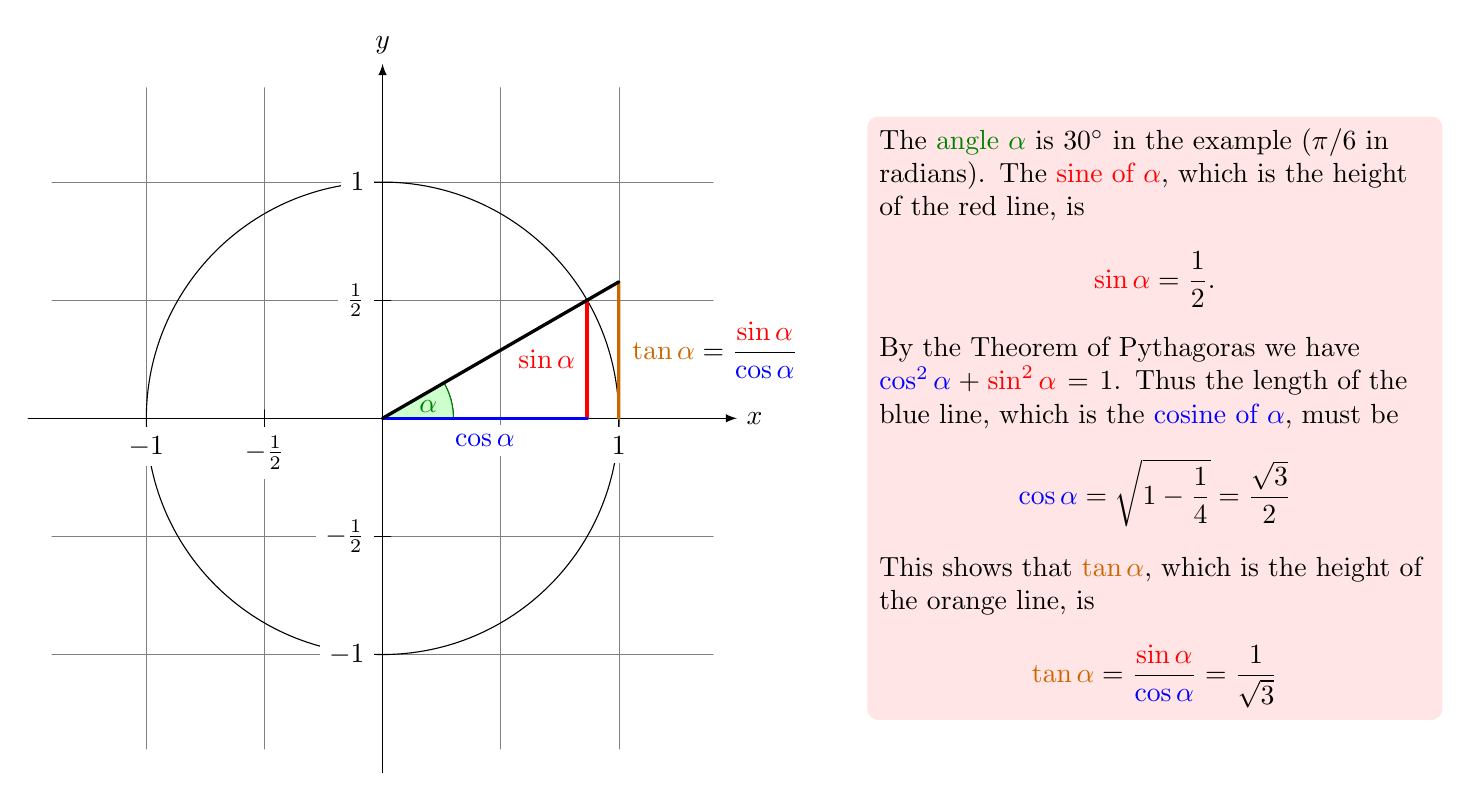
\begin{tikzpicture}[
    scale=3,
    line cap=round,
    %styles
    axes/.style=,
    important line/.style={very thick},
    information text/.style={rounded corners,fill=red!10,inner sep=1ex},
  ]
  %colors
  \colorlet{anglecolor}{green!50!black}
  \colorlet{sincolor}{red}
  \colorlet{tancolor}{orange!80!black}
  \colorlet{coscolor}{blue}
  \draw[step=.5cm,gray,very thin] (-1.4,-1.4) grid (1.4,1.4);
  \draw (0,0) circle [radius=1cm];

  \begin{scope}[axes]
    \draw[-latex] (-1.5,0) -- (1.5,0) node[right] {$x$} coordinate(x axis);
    \draw[-latex] (0,-1.5) -- (0,1.5) node[above] {$y$} coordinate(y axis);
    \foreach \x/\xtext in {-1, -0.5/-\frac{1}{2},1}
    \draw (\x cm,1pt) -- (\x cm,-1pt) node[anchor=north,fill=white] {$\xtext$};
    \foreach \y/\ytext in {-1, -0.5/-\frac{1}{2}, 0.5/\frac{1}{2}, 1}
    \draw (1pt,\y cm) -- (-1pt,\y cm) node[anchor=east,fill=white] {$\ytext$};
  \end{scope}
  \draw (3mm,0mm) arc [start angle=0, end angle=30, radius=3mm];
  \filldraw[fill=green!20!white, draw=green!50!black] (0,0) -- (3mm,0mm) arc [start angle=0, end angle=30, radius=3mm] -- cycle;
  \draw (15:2mm) node[anglecolor] {$\alpha$};
  \draw[important line,sincolor]
  (30:1cm) -- node[left=.5pt,fill=white] {$\sin \alpha$} (30:1cm |- x axis);
  %标注\sin的位置为 (30:1cm |- x axis) -- (30:1cm)路径的中点
  \draw[important line,coscolor]
  (30:1cm |- x axis) -- node[below=2pt,fill=white] {$\cos \alpha$} (0,0);
  %标注\cos的位置为 (30:1cm |- x axis) -- (0,0)路径的中点
  \path [name path=upward line] (1,0) -- (1,1);
  \path [name path=sloped line] (0,0) -- (30:1.5cm);
  \draw [name intersections={of=upward line and sloped line, by=x}]
  [important line,tancolor] (1,0) -- node [right=1pt,fill=white]
  {$\displaystyle \tan \alpha \color{black}=
      \frac{{\color{red}\sin \alpha}}{\color{blue}\cos \alpha}$} (x);
  %标注\tan的位置为 (1,0) -- (x) 路径的中点
  \draw[very thick] (0,0) -- (x);

  \draw[xshift=2.05cm]
  node[right,text width=7cm,information text]
  {
  The {\color{anglecolor} angle $\alpha$} is $30^\circ$ in the
  example ($\pi/6$ in radians). The {\color{sincolor}sine of
      $\alpha$}, which is the height of the red line, is
  \[
    {\color{sincolor} \sin \alpha} = \frac{1}{2}.
  \]
  By the Theorem of Pythagoras we have ${\color{coscolor} \cos^2\alpha} + {\color{sincolor}\sin^2\alpha} =1$. Thus the length of the blue line, which is the {\color{coscolor}cosine of $\alpha$}, must be
  $$
    {\color{coscolor}\cos\alpha} = \sqrt{1-\frac{1}{4}} = \frac{\sqrt{3}}{2}
  $$
  This shows that {\color{tancolor}$\tan\alpha$}, which is the height of the orange line, is
  $$
    {\color{tancolor}\tan\alpha} = \frac{{\color{sincolor}\sin\alpha}}{{\color{coscolor}\cos\alpha}} = \frac{1}{\sqrt{3}}
  $$
  };
\end{tikzpicture}

\task{A Petri-Net for Hagen}
\scalebox{.6}{
  \includegraphics{./fig/figure2.png}
}

\step{设置需要调用的\wordbox{TIKZ}库和子图基本框架}
\begin{tikzpicture}
  %使用\node命令绘制具有五个节点的子图
  \node at (0,2) [circle,draw] {};
  \node at (0,1) [circle,draw] {};
  \node at (0,0) [circle,draw] {};
  \node at (1,1) [rectangle,draw] {};
  \node at (-1,1) [rectangle,draw] {};
\end{tikzpicture}

\step{添加粗细\wordbox{thick}并设置颜色样式\wordbox{draw}与\wordbox{fill}选项}
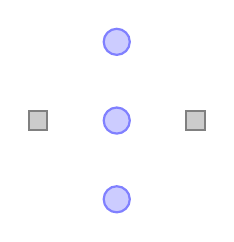
\begin{tikzpicture}[thick]
  %使用\node命令绘制具有五个节点的子图
  \node at (0,2) [circle,draw=blue!50,fill=blue!20] {};
  \node at (0,1) [circle,draw=blue!50,fill=blue!20] {};
  \node at (0,0) [circle,draw=blue!50,fill=blue!20] {};
  \node at (1,1) [rectangle,draw=black!50,fill=black!20] {};
  \node at (-1,1) [rectangle,draw=black!50,fill=black!20] {};
\end{tikzpicture}

\step{使用\wordbox{tikz.style}实现代码复用,并设置\wordbox{minimize size}增大node内部间距}
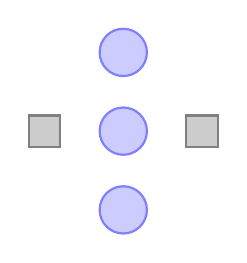
\begin{tikzpicture}
  [
    place/.style={circle,draw=blue!50,fill=blue!20,thick,inner sep=0pt,minimum size=6mm},
    transition/.style={rectangle,draw=black!50,fill=black!20,thick,inner sep=0pt,minimum size=4mm}
  ]
  \node at (0,2) [place] {};
  \node at (0,1) [place] {};
  \node at (0,0) [place] {};
  \node at (1,1) [transition] {};
  \node at (-1,1) [transition] {};
\end{tikzpicture}

\step{任意调整\wordbox{node}的\wordbox{syntax}位置并设置坐标点名称}
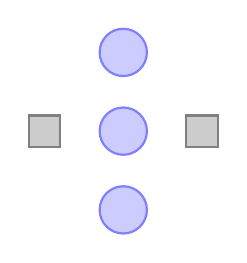
\begin{tikzpicture}
  [
    place/.style={circle,draw=blue!50,fill=blue!20,thick,inner sep=0pt,minimum size=6mm},
    transition/.style={rectangle,draw=black!50,fill=black!20,thick,inner sep=0pt,minimum size=4mm}
  ]
  \node[place] at (0,2) (waiting 1) {};
  \node[place] at (0,1) (critical 1) {};
  \node[place] at (0,0) (semaphore) {};
  \node[transition] at (1,1) (leave critical) {};
  \node[transition] at (-1,1) (enter critical) {};
\end{tikzpicture}

\step{弃用坐标而改用相对位置参数\wordbox{above}、\wordbox{below}、\wordbox{left}、\wordbox{right}表示各\wordbox{node}间相互关系}
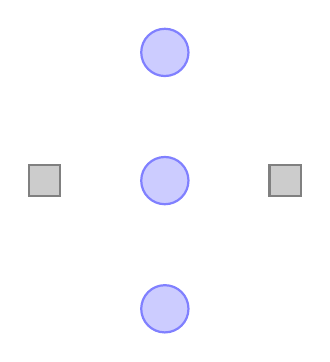
\begin{tikzpicture}
  [
    place/.style={circle,draw=blue!50,fill=blue!20,thick,inner sep=0pt,minimum size=6mm},
    transition/.style={rectangle,draw=black!50,fill=black!20,thick,inner sep=0pt,minimum size=4mm}
  ]
  \node[place] (waiting) {};
  \node[place] (critical) [below = of waiting] {};
  \node[place] (semaphore) [below = of critical] {};
  \node[transition] (leave critical) [right = of critical] {};
  \node[transition] (enter critical) [left = of critical] {};
\end{tikzpicture}

\step{使用\wordbox{label}(可以用多个)添加\wordbox{label}选项进行标注,并在全局label选项中使用\wordbox{every}定义标注样式}
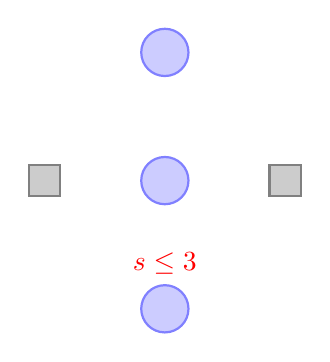
\begin{tikzpicture}
  [
    every label/.style={red},
    place/.style={circle,draw=blue!50,fill=blue!20,thick,inner sep=0pt,minimum size=6mm},
    transition/.style={rectangle,draw=black!50,fill=black!20,thick,inner sep=0pt,minimum size=4mm}
  ]
  \node[place] (waiting) {};
  \node[place] (critical) [below = of waiting] {};
  \node[place] (semaphore) [below = of critical,
    label = above:$s\le3$] {};
  \node[transition] (leave critical) [right = of critical] {};
  \node[transition] (enter critical) [left = of critical] {};
\end{tikzpicture}

\step{尝试使用控制点增加\wordbox{node}间的链接箭头,但控制点的距离较难精确把控}
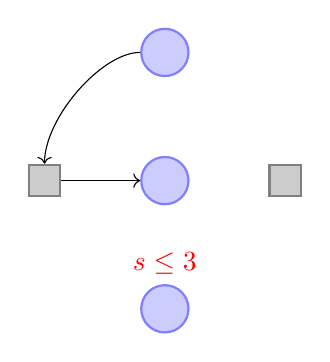
\begin{tikzpicture}
  [
    every label/.style={red},
    place/.style={circle,draw=blue!50,fill=blue!20,thick,inner sep=0pt,minimum size=6mm},
    transition/.style={rectangle,draw=black!50,fill=black!20,thick,inner sep=0pt,minimum size=4mm}
  ]
  \node[place] (waiting) {};
  \node[place] (critical) [below = of waiting] {};
  \node[place] (semaphore) [below = of critical,
    label = above:$s\le3$] {};
  \node[transition] (leave critical) [right = of critical] {};
  \node[transition] (enter critical) [left = of critical] {};
  \draw [->] (enter critical) -- (critical);
  \draw [->] (waiting) .. controls +(left:8mm)  and +(up:8mm)
  .. (enter critical);
\end{tikzpicture}

\step{使用\wordbox{to}命令并指定\wordbox{out}与\wordbox{in}选项控制箭头的输入输出角度,也可以使用\wordbox{bend left/right}命令直接指定圆弧状箭头的方向}
可以得到更加饱满圆角的弧线箭头(嘿嘿)

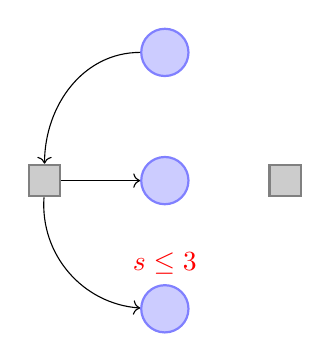
\begin{tikzpicture}
  [
    every label/.style={red},
    place/.style={circle,draw=blue!50,fill=blue!20,thick,inner sep=0pt,minimum size=6mm},
    transition/.style={rectangle,draw=black!50,fill=black!20,thick,inner sep=0pt,minimum size=4mm}
  ]
  \node[place] (waiting) {};
  \node[place] (critical) [below = of waiting] {};
  \node[place] (semaphore) [below = of critical,
    label = above:$s\le3$] {};
  \node[transition] (leave critical) [right = of critical] {};
  \node[transition] (enter critical) [left = of critical] {};
  \draw [->] (enter critical) to (critical);
  \draw [->] (waiting) to [out=180,in=90] (enter critical);
  \draw [->] (enter critical) to [bend right=45] (semaphore);
\end{tikzpicture}

\step{使用\wordbox{node}的\wordbox{edge}选项更优雅地一次性指定箭头指向}

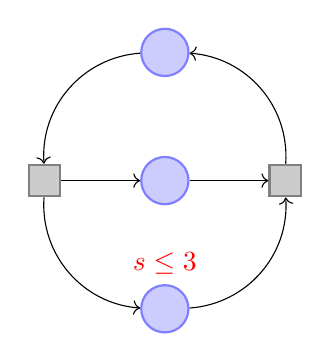
\begin{tikzpicture}
  [
  place/.style={circle,draw=blue!50,fill=blue!20,thick,inner sep=0pt,minimum size=6mm},
  transition/.style={rectangle,draw=black!50,fill=black!20,thick,inner sep=0pt,minimum size=4mm},
  every label/.style={red},bend angle=45,
  pre/.style={<-,shorten <=1pt,>={Stealth[round]},semithick},
  post/.style={->,shorten >=1pt,>={Stealth[round]},semithick}
  ]
  \node[place] (waiting) {};
  \node[place] (critical) [below = of waiting] {};
  \node[place] (semaphore) [below = of critical,
    label = above:$s\le3$] {};
  \node[transition] (leave critical) [right = of critical] {}
  edge[<-] (critical)
  edge[<-,bend left=45] (semaphore)
  edge[->,bend right=45] (waiting);
  \node[transition] (enter critical) [left = of critical] {}
  edge[->] (critical)
  edge[->,bend right=45] (semaphore)
  edge[<-,bend left=45] (waiting);
\end{tikzpicture}

\step{使用\wordbox{pre}与\wordbox{post}的箭头样式并绘制整个子图框架}
同时如法炮制绘制出整个子图的整体框架

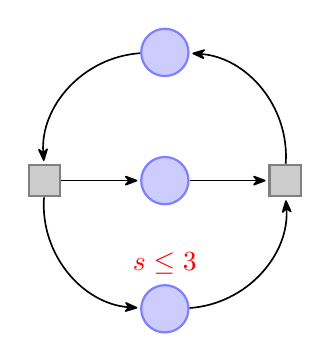
\begin{tikzpicture}
  [
  place/.style={circle,draw=blue!50,fill=blue!20,thick,inner sep=0pt,minimum size=6mm},
  transition/.style={rectangle,draw=black!50,fill=black!20,thick,inner sep=0pt,minimum size=4mm},
  every label/.style={red},bend angle=45,
  pre/.style={<-,shorten <=1pt,>={Stealth[round]},semithick},
  post/.style={->,shorten >=1pt,>={Stealth[round]},semithick}
  ]
  \node[place] (waiting) {};
  \node[place] (critical) [below = of waiting] {};
  \node[place] (semaphore) [below = of critical,
    label = above:$s\le3$] {};
  \node[transition] (leave critical) [right = of critical] {}
  edge[pre] (critical)
  edge[pre,bend left] (semaphore)
  edge[post,bend right] (waiting);
  \node[transition] (enter critical) [left = of critical] {}
  edge[post] (critical)
  edge[post,bend right] (semaphore)
  edge[pre,bend left] (waiting);
\end{tikzpicture}

\step{使用\wordbox{node}添加文字标注,并利用\wordbox{scope}环境选项\wordbox{on background layer}添加阴影}
其中\wordbox{auto}用于自动确定标注位置,\wordbox{swap}用于放置到现有位置的镜像对称位置(此处使用\wordbox{swap}后数字标注将从内侧移动到外侧).

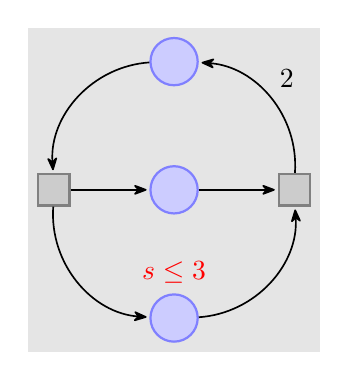
\begin{tikzpicture}
  [
  place/.style={circle,draw=blue!50,fill=blue!20,thick,inner sep=0pt,minimum size=6mm},
  transition/.style={rectangle,draw=black!50,fill=black!20,thick,inner sep=0pt,minimum size=4mm},
  every label/.style={red},bend angle=45,
  pre/.style={<-,shorten <=1pt,>={Stealth[round]},semithick},
  post/.style={->,shorten >=1pt,>={Stealth[round]},semithick}
  ]
  \node[place] (waiting) {};
  \node[place] (critical) [below = of waiting] {};
  \node[place] (semaphore) [below = of critical,
    label = above:$s\le3$] {};
  \node[transition] (leave critical) [right = of critical] {}
  edge[pre] (critical)
  edge[pre,bend left] (semaphore)
  edge[post,bend right] node [auto,swap] {2} (waiting);
  \node[transition] (enter critical) [left = of critical] {}
  edge[post] (critical)
  edge[post,bend right] (semaphore)
  edge[pre,bend left] (waiting);
  \begin{scope}[on background layer]
    \node [fill=black!10,fit=(waiting) (critical) (semaphore) (leave critical) (enter critical)] {};
  \end{scope}
\end{tikzpicture}

\step{小彩蛋:基于\wordbox{decorations.pathmorphing}绘制蛇形箭头}
\begin{itemize}
  \item {指定\wordbox{decorate}与\wordbox{decoration=snake}选项绘制蛇形箭头.\\
        \tikz\draw[->,decorate,decoration=snake] (0,0) -- (3,0);}
  \item {指定选项\wordbox{amplitude},\wordbox{amplitude}以及\wordbox{amplitude}指定蛇形路径的弯曲程度、长度等参数.\\
        \tikz\draw[->,decorate,decoration={
              snake,
              amplitude=.4mm,
              segment length=2mm,
              post length=1mm}
        ] (0,0) -- (3,0);}
  \item {指定\wordbox{node}选项\wordbox{text width}实现自动换行,指定\wordbox{midway}设置标注位置为当前路径中点.\\
        \tikz\draw [->,decorate,decoration={snake,
              amplitude=.4mm,segment length=2mm,post length=1mm}] (0,0) -- (3,0)
        node [above,text width=3cm,align=center,midway] {replacement of the \textcolor{red}{capacity} by \textcolor{red}{two places}};
        }
\end{itemize}

\step{补充部分细节绘制左半图形}
\begin{itemize}
  \item 设置\wordbox{node diatance}、\wordbox{on grid}选项控制图片样式
  \item 设置选项\wordbox{tokens}选择控制生成点数
  \item 完善左图的其他交点与连线图形
\end{itemize}

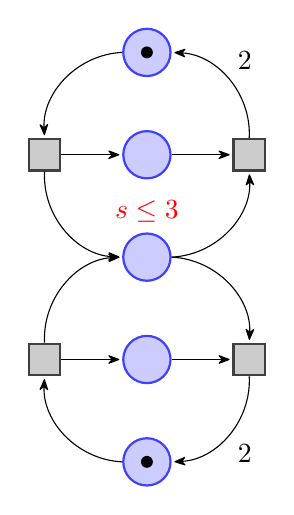
\begin{tikzpicture}[
  node distance=1.3cm,
  on grid,auto,bend angle=45,
  >={Stealth[round]},
  every place/.style= {minimum size=6mm,thick,draw=blue!75,fill=blue!20},
  red place/.style= {place,draw=red!75,fill=red!20},
  every transition/.style={thick,draw=black!75,fill=black!20},
  every label/.style= {red}]
  % w-waiting c-critical s-semaphore e-enter l-leave
  \node [place,tokens=1] (w1) {};
  \node [place]          (c1) [below = of w1] {};
  \node [place]          (s)  [below=of c1,
    label=above:$s\le 3$] {};
  \node [place]          (c2) [below=of s] {};
  \node [place,tokens=1] (w2) [below=of c2] {};
  \node [transition] (e1) [left = of c1] {}
  edge [pre, bend left] (w1)
  edge [post] (c1)
  edge [post, bend right] (s);
  \node [transition] (e2) [left = of c2] {}
  edge [pre, bend right] (w2)
  edge [post] (c2)
  edge [post, bend left] (s);
  \node [transition] (l1) [right = of c1] {}
  edge [post, bend right] node[swap] {2} (w1)
  edge [pre] (c1)
  edge [pre, bend left] (s);
  \node [transition] (l2) [right = of c2] {}
  edge [post, bend left] node {2} (w2)
  edge [pre] (c2)
  edge [pre, bend right] (s);
\end{tikzpicture}

\step{如法炮制绘制右半部分图}
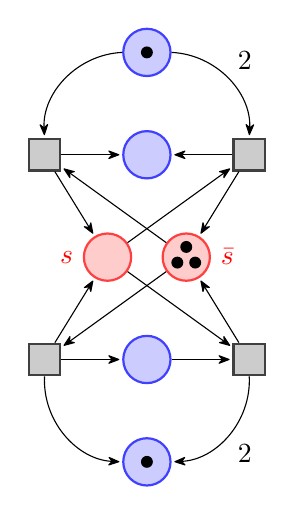
\begin{tikzpicture}[
  node distance=1.3cm,
  on grid,auto,bend angle=45,
  >={Stealth[round]},
  every place/.style= {minimum size=6mm,thick,draw=blue!75,fill=blue!20},
  red place/.style= {place,draw=red!75,fill=red!20},
  every transition/.style={thick,draw=black!75,fill=black!20},
  every label/.style= {red}]
  % w-waiting c-critical s-semaphore e-enter l-leave
  \node [place,tokens=1] (w1') {};
  \node [place]          (c1') [below = of w1'] {};
  \node [red place]      (s1') [below = of c1', xshift=-5mm] [label=left:$s$] {};
  \node [red place,tokens=3] (s2') [below=of c1',xshift=5mm] [label=right:$\bar{s}$] {};
  %注意此处shift了,所以node—S2的位置需要逆向shift=+5mm
  \node [place] (c2') [below=of s1',xshift=5mm] {};
  \node [place,tokens=1] (w2') [below=of c2'] {};
  \node [transition] (e1') [left = of c1'] {}
  edge [pre,bend left]   (w1')
  edge [post]            (s1')
  edge [pre]             (s2')
  edge [post]            (c1');
  \node [transition] (l1') [right = of c1'] {}
  edge [pre, bend right] node[swap] {2} (w1')
  edge [post] (c1')
  edge [pre] (s1')
  edge [post] (s2');
  \node [transition] (e2') [left=of c2'] {}
  edge [post] (c2')
  edge [post] (s1')
  edge [pre] (s2')
  edge [post,bend right] (w2');
  \node [transition] (l2') [right=of c2'] {}
  edge [pre] (c2')
  edge [pre] (s1')
  edge [post] (s2')
  edge [post,bend left] node {2} (w2');
\end{tikzpicture}

\step{合并上述所有代码,利用\wordbox{scope}环境实现\wordbox{xshift}位移并添加阴影,最后利用\wordbox{decoration=snake}添加蛇形箭头.[\wordbox{full code}]}
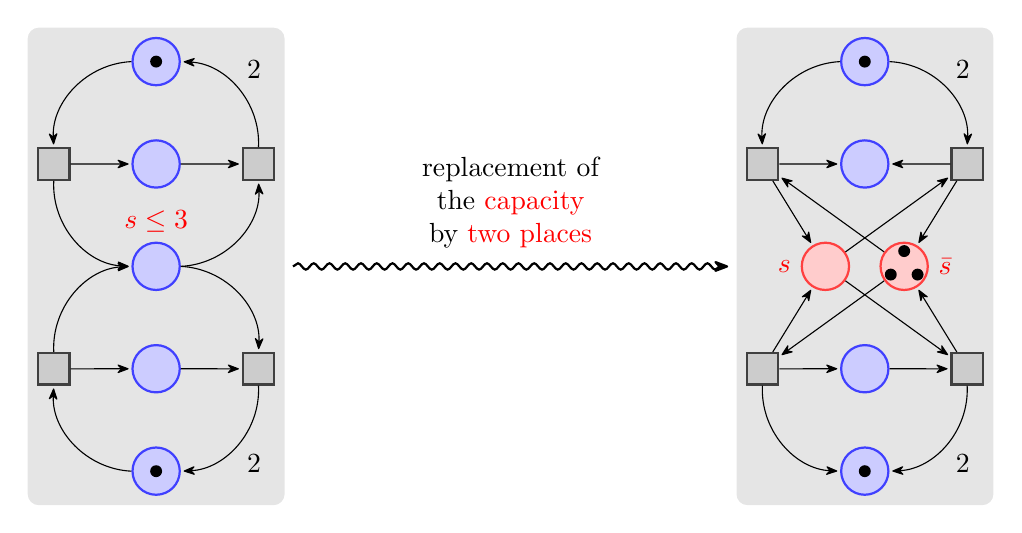
\begin{tikzpicture}[
  node distance=1.3cm,scale=1.5,
  on grid,auto,bend angle=45,
  >={Stealth[round]},
  every place/.style= {minimum size=6mm,thick,draw=blue!75,fill=blue!20},
  red place/.style= {place,draw=red!75,fill=red!20},
  every transition/.style={thick,draw=black!75,fill=black!20},
  every label/.style= {red}
  ]
  % w-waiting c-critical s-semaphore e-enter l-leave
  \node [place,tokens=1] (w1) {};
  \node [place]          (c1) [below = of w1] {};
  \node [place]          (s)  [below=of c1,
    label=above:$s\le 3$] {};
  \node [place]          (c2) [below=of s] {};
  \node [place,tokens=1] (w2) [below=of c2] {};
  \node [transition] (e1) [left = of c1] {}
  edge [pre, bend left] (w1)
  edge [post] (c1)
  edge [post, bend right] (s);
  \node [transition] (e2) [left = of c2] {}
  edge [pre, bend right] (w2)
  edge [post] (c2)
  edge [post, bend left] (s);
  \node [transition] (l1) [right = of c1] {}
  edge [post, bend right] node[swap] {2} (w1)
  edge [pre] (c1)
  edge [pre, bend left] (s);
  \node [transition] (l2) [right = of c2] {}
  edge [post, bend left] node {2} (w2)
  edge [pre] (c2)
  edge [pre, bend right] (s);
  \begin{scope}[xshift=6cm]
    % w-waiting c-critical s-semaphore e-enter l-leave
    \node [place,tokens=1] (w1') {};
    \node [place]          (c1') [below = of w1'] {};
    \node [red place]      (s1') [below = of c1', xshift=-5mm] [label=left:$s$] {};
    \node [red place,tokens=3] (s2') [below=of c1',xshift=5mm] [label=right:$\bar{s}$] {};
    %注意此处shift了,所以node—S2的位置需要逆向shift=+5mm
    \node [place] (c2') [below=of s1',xshift=5mm] {};
    \node [place,tokens=1] (w2') [below=of c2'] {};
    \node [transition] (e1') [left = of c1'] {}
    edge [pre,bend left]   (w1')
    edge [post]            (s1')
    edge [pre]             (s2')
    edge [post]            (c1');
    \node [transition] (l1') [right = of c1'] {}
    edge [pre, bend right] node[swap] {2} (w1')
    edge [post] (c1')
    edge [pre] (s1')
    edge [post] (s2');
    \node [transition] (e2') [left=of c2'] {}
    edge [post] (c2')
    edge [post] (s1')
    edge [pre] (s2')
    edge [post,bend right] (w2');
    \node [transition] (l2') [right=of c2'] {}
    edge [pre] (c2')
    edge [pre] (s1')
    edge [post] (s2')
    edge [post,bend left] node {2} (w2');
  \end{scope}
  \begin{scope}[on background layer]
    \node (r1) [fill=black!10,rounded corners,fit=(w1)(w2)(e1)(e2)(l1)(l2)] {};
    \node (r2) [fill=black!10,rounded corners,fit=(w1')(w2')(e1')(e2')(l1')(l2')] {};
  \end{scope}
  %添加蛇形箭头
  \draw [shorten >=1mm,->,thick,decorate,decoration={snake,amplitude=.4mm,segment length=2mm,pre=moveto,pre length=1mm,post length=2mm}] (r1) -- (r2) node [above=1mm,midway,text width=3cm,align=center] {replacement of the \textcolor{red}{capacity} by \textcolor{red}{two places}};
\end{tikzpicture}

\task{Euclid's Amber Version of the Elements}
\scalebox{.6}{
  \includegraphics{./fig/figure3.png}
}

\step{使用\wordbox{label}选项优雅地绘制线段\wordbox{$AB$}}
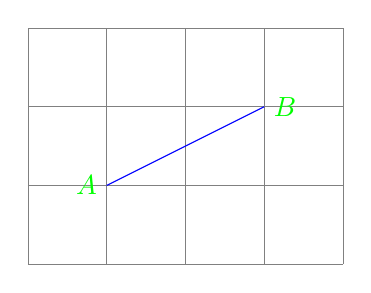
\begin{tikzpicture}
  \draw[help lines] (-1,-1) grid (3,2);
  \coordinate [label=left:\textcolor{green}{$A$}] (A) at (0,0);
  \coordinate [label=right:\textcolor{green}{$B$}] (B) at (2,1);
  \draw[blue] (A) -- (B);
\end{tikzpicture}
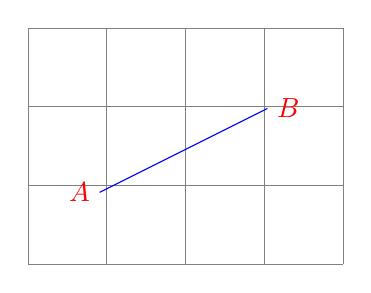
\begin{tikzpicture}
  \draw[help lines] (-1,-1) grid (3,2);
  \coordinate [label=left:\textcolor{red}{$A$}] (A) at (0+0.1*rand,0-0.1*rand);
  \coordinate [label=right:\textcolor{red}{$B$}] (B) at (2-0.1*rand,1+0.2*rand);
  \draw[blue] (A) -- (B);
\end{tikzpicture}
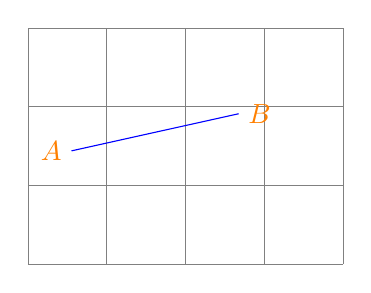
\begin{tikzpicture}
  \draw[help lines] (-1,-1) grid (3,2);
  \coordinate [label=left:\textcolor{orange}{$A$}] (A) at ($(0,0) + .5*(rand,rand) $);
  \coordinate [label=right:\textcolor{orange}{$B$}] (B) at ($(2,1) + .8*(rand,rand) $);
  \draw[blue] (A) -- (B);
\end{tikzpicture}

\step{使用\wordbox{let<digit>}关键字获取坐标,使用\wordbox{veclen}计算距离}
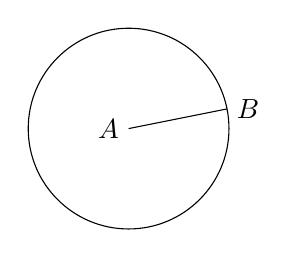
\begin{tikzpicture}
  \coordinate [label=left:$A$] (A) at (0,0);
  \coordinate [label=right:$B$] (B) at (1.25,0.25);
  \draw (A) -- (B);
  \draw (A) let \p1 = ($(B)-(A)$) in circle ({veclen(\x1,\y1)});
\end{tikzpicture}

注意在使用坐标计算模式时需要使用(\$ \$)包围,同时指定数字时需要使用大括号\{ \}包围.

\step{更进一步利用\wordbox{let}指定的坐标同时绘制两个圆}
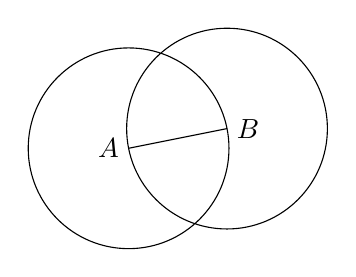
\begin{tikzpicture}
  \coordinate [label=left:$A$] (A) at (0,0);
  \coordinate [label=right:$B$] (B) at (1.25,0.25);
  \draw (A) -- (B);
  \draw let
  \p1 = ($(B)-(A)$),%woc这里let的赋值语句间需使用逗号分隔
  \n2 = {veclen(\x1,\y1)}
  in
  (A) circle (\n2)
  (B) circle (\n2);
\end{tikzpicture}

\step{使用\wordbox{circle through}标注圆上的其他点}
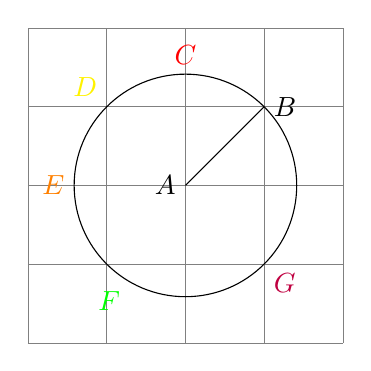
\begin{tikzpicture}
  \draw [help lines] (-2,-2) grid (2,2);
  \coordinate [label=left:$A$] (A) at (0,0);
  \coordinate [label=right:$B$] (B) at (1,1);
  \draw (A) -- (B);
  \node [draw,circle through=(B),
    label=above:\textcolor{red}{$C$},
    label=135:\textcolor{yellow}{$D$},
    label=left:\textcolor{orange}{$E$},
    label=240:\textcolor{green}{$F$},
    label=315:\textcolor{purple}{$G$}] at (A) {};
\end{tikzpicture}

\step{使用\wordbox{name path/intersection}指定路径与路径的交点}
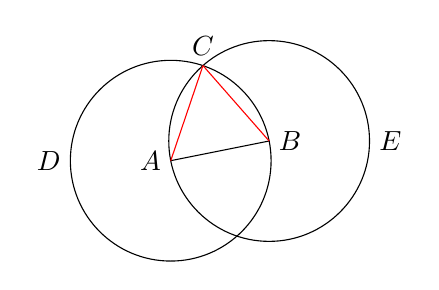
\begin{tikzpicture}
  \coordinate [label=left:$A$] (A) at (0,0);
  \coordinate [label=right:$B$] (B) at (1.25,0.25);
  \draw (A) -- (B);
  \node (D) [name path=D,draw,circle through=(B),label=left:$D$] at (A) {};
  \node (E) [name path=E,draw,circle through=(A),label=right:$E$] at (B) {};
  % Name the coordinates, but do not draw anything:
  \path [name intersections={of=D and E}];%默认使用 intersection-<digit>形式命名交点
  \coordinate [label=above:$C$] (C) at (intersection-1);
  \draw [red] (A) -- (C);
  \draw [red] (B) -- (C);
\end{tikzpicture}

\step{借助\wordbox{by}进一步简化代码并进行交点标注}
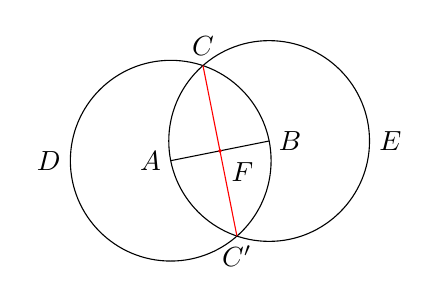
\begin{tikzpicture}
  \coordinate [label=left:$A$] (A) at (0,0);
  \coordinate [label=right:$B$] (B) at (1.25,0.25);
  \draw [name path=A--B] (A) -- (B);
  \node (D) [name path=D,draw,circle through=(B),label=left:$D$] at (A) {};
  \node (E) [name path=E,draw,circle through=(A),label=right:$E$] at (B) {};
  %此处的D E指的是圆的路径,故其交点为C C' 当有多个交点时,可使用by={<P1>,<P2>,...,<Pn>指定}
  \path [name intersections={of=D and E, by={[label=above:$C$]C, [label=below:$C'$]C'}}];
  \draw [name path=C--C',red] (C) -- (C');
  \path [name intersections={of=A--B and C--C',by=F}];
  \node [circle,fill=red,inner sep=.5pt,label=-45:$F$] at (F) {};
\end{tikzpicture}

\step{更进一步完善左半图的代码}
\begin{itemize}
  \item 在tikzpicture环境中添加help lines选项
  \item 使用colorlet命令自定义颜色
  \item 使用PlainTex命令def定义输入节点文本的命令
  \item 使用foreach命令遍历目标点序列A,B,C,并添加阴影
  \item 使用pgfonlayer命令在背景层绘制橙色三角形
\end{itemize}
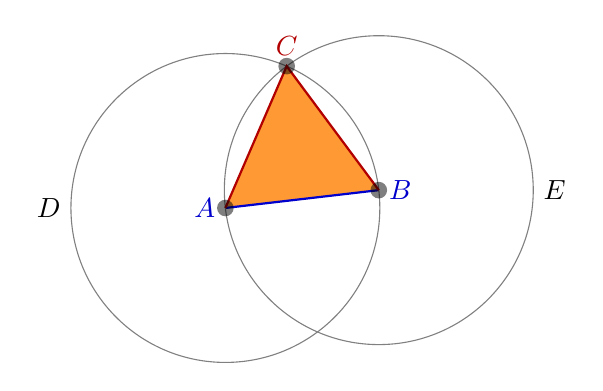
\begin{tikzpicture}[
    thick,scale=1.5,help lines/.style={thin,draw=black!50}
  ]
  \def\A{\textcolor{input}{$A$}}
  \def\B{\textcolor{input}{$B$}}
  \def\C{\textcolor{output}{$C$}}
  \def\D{$D$} \def\E{$E$}
  \colorlet{input}{blue!80!black}
  \colorlet{output}{red!70!black}
  \colorlet{triangle}{orange}
  \coordinate [label=left:\A] (A) at ($ (0,0) + .1*(rand,rand) $);
  \coordinate [label=right:\B] (B) at ($ (1.25,0.25) + .1*(rand,rand) $);
  \draw [input] (A) -- (B);
  \node [name path=D,help lines,draw,label=left:\D] (D) at (A) [circle through=(B)] {};
  \node [name path=E,help lines,draw,label=right:\E] (E) at (B) [circle through=(A)] {};
  \path [name intersections={of=D and E,by={[label=above:\C]C}}];
  \draw [output] (A) -- (C) -- (B);
  \foreach \point in {A,B,C}
  \fill [black,opacity=.5] (\point) circle (2pt);
  \begin{pgfonlayer}{background}%
    \fill[triangle!80] (A) -- (C) -- (B) -- cycle;
  \end{pgfonlayer}
\end{tikzpicture}

下面让我们进入右半部分图片的绘制嘿嘿.

\step{使用两种\wordbox{Partway Calculations}获取点的变换点}

\textbf{方法一:}(坐标比例定点法)需要在数学计算模式(\$...\$)中使用\wordbox{(Point1)!<scale>!(Point2)}计算线段的中间点.

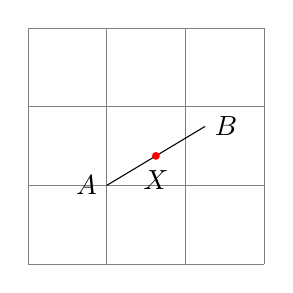
\begin{tikzpicture}
  \draw[help lines] (-1,-1) grid (2,2);
  \coordinate [label=left:$A$] (A) at (0,0);
  \coordinate [label=right:$B$] (B) at (1.25,0.75);
  \draw (A) -- (B);
  \node [circle,fill=red,inner sep=1pt,label=below:$X$] (X) at ($ (A)!.5!(B) $) {};
\end{tikzpicture}

\textbf{方法二:}(旋转拉伸定点法)在数学计算模式(\$...\$)中使用\wordbox{(Point1)!<proportion>!<angle>:(Point2)}计算点2绕点1顺时针旋转<angle>角度之后拉伸<scale>倍的位置.

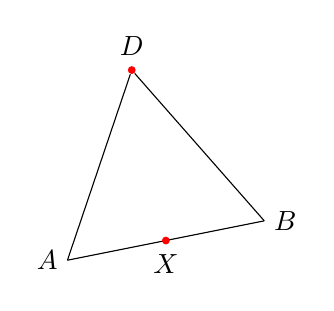
\begin{tikzpicture}[scale=2]
  \coordinate [label=left:$A$] (A) at (0,0);
  \coordinate [label=right:$B$] (B) at (1.25,0.25);
  \draw (A) -- (B);
  \node [circle,fill=red,inner sep=1pt,label=below:$X$] (X) at ($ (A)!.5!(B) $) {};
  \node [circle,fill=red,inner sep=1pt,label=above:$D$] (D) at ($ (X) ! {sin(60)*2} ! 90:(B) $) {};
  \draw (A) -- (D) -- (B);
\end{tikzpicture}

\step{精彩再现:再次使用circle through标注圆周上的点}
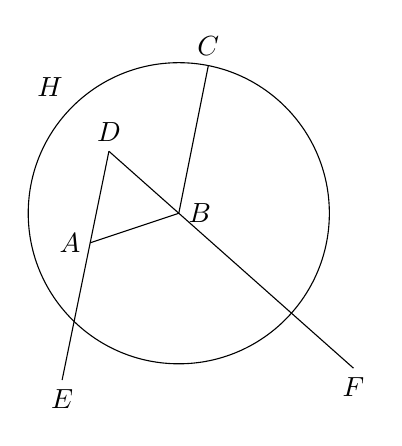
\begin{tikzpicture}[scale=1.5]
  \coordinate[label=left:$A$] (A) at (0,0);
  \coordinate[label=right:$B$] (B) at (.75,.25);
  \coordinate[label=above:$C$] (C) at (1,1.5);
  \draw (A) -- (B) -- (C);
  % D 点为以 AB 为一条边的等边三角形
  \coordinate[label=above:$D$] (D) at ($(A)! 1 !60:(B)$);
  % 以 B 为圆心 BC 为半径的圆周上标记点 H
  \node (H) [draw,label=135:$H$,circle through=(C)] at (B) {};%本行的draw绘制了圆
  \draw (D) -- ($(D) ! 2.5 ! (A)$) coordinate [label=below:$E$] (E);
  \draw (D) -- ($(D) ! 3.5 ! (B)$) coordinate [label=below:$F$] (F);
\end{tikzpicture}

\step{小彩蛋:使用\wordbox{intersection}定点并添加使用\wordbox{opacity}添加半透明阴影点}
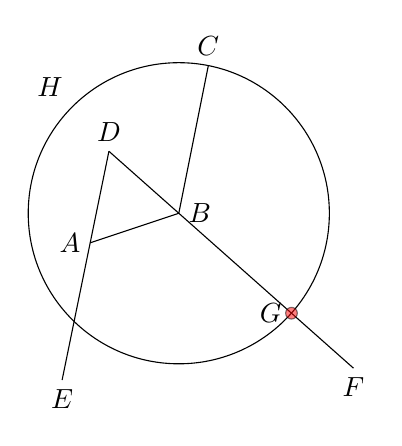
\begin{tikzpicture}[scale=1.5]
  \coordinate[label=left:$A$] (A) at (0,0);
  \coordinate[label=right:$B$] (B) at (.75,.25);
  \coordinate[label=above:$C$] (C) at (1,1.5);
  \draw (A) -- (B) -- (C);
  % D 点为以 AB 为一条边的等边三角形
  \coordinate[label=above:$D$] (D) at ($(A)! 1 !60:(B)$);
  % 以 B 为圆心 BC 为半径的圆周上标记点 H
  \node (H) [name path=H,draw,label=135:$H$,circle through=(C)] at (B) {};%本行的draw绘制了圆
  \draw (D) -- ($(D) ! 2.5 ! (A)$) coordinate [label=below:$E$] (E);
  \draw (D) -- ($(D) ! 3.5 ! (B)$) coordinate [label=below:$F$] (F);
  %给 BF 与圆周的交点添加半透明红色node
  \path[name path=B--F] (B) -- (F);
  \path[name intersections={of = H and B--F,by ={[label=left:$G$]G}}];
  \node[draw,circle,fill=red,opacity=0.5,inner sep=1.5pt] at (G) {};
\end{tikzpicture}

\step{一鼓作气搞定右半图形}
\begin{itemize}
  \item 使用\wordbox{def}结合\wordbox{colorlet}命令共同调用颜色
  \item 使用\wordbox{name path/intersections}绘制圆的路径与交点
  \item 使用\wordbox{foreach}结合\wordbox{opacity}绘制阴影点
\end{itemize}
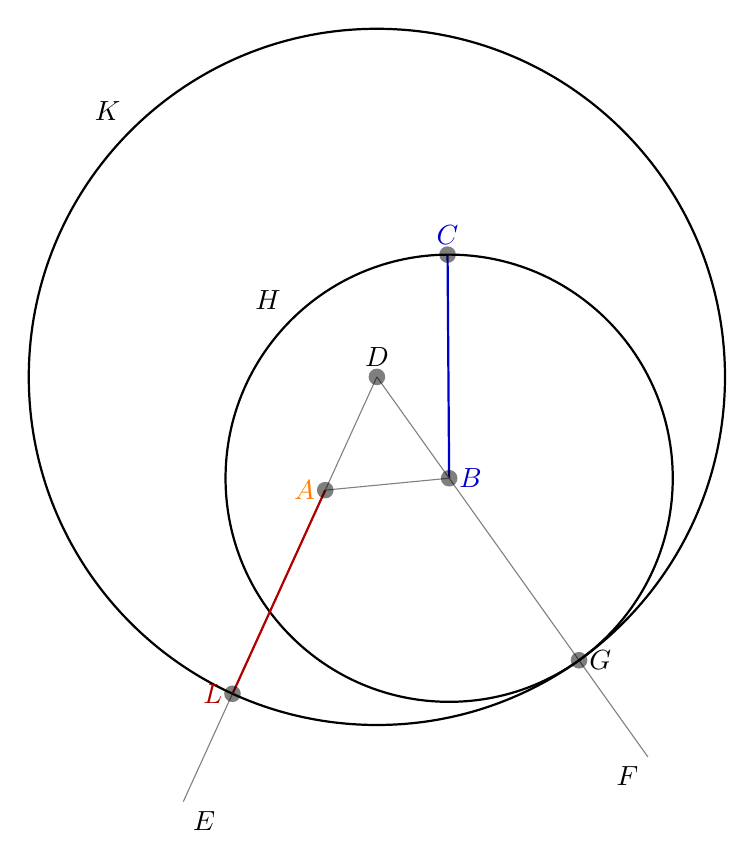
\begin{tikzpicture}[scale=1.5,thick,help lines/.style={thin,draw=black!50}]
  \def\A{\textcolor{fill}{$A$}}
  \def\B{\textcolor{input}{$B$}}
  \def\C{\textcolor{input}{$C$}}
  \def\D{$D$}\def\E{$E$}\def\F{$F$}
  \def\G{$G$}\def\H{$H$}\def\K{$K$}
  \def\L{\textcolor{output}{$L$}}
  \colorlet{fill}{orange}
  \colorlet{input}{blue!80!black}
  \colorlet{output}{red!70!black}
  \coordinate [label=left:\A] (A) at
  ($(0,0) + .1*(rand,rand) $);
  \coordinate [label=right:\B] (B) at
  ($(1,.2) + .1*(rand,rand) $);
  \coordinate [label=above:\C] (C) at
  ($(1,2) + .1*(rand,rand) $);
  \draw[input] (B)--(C);
  \draw[help lines] (A) -- (B);
  %使用旋转缩放定点法计算点D的坐标
  \coordinate [label=above:\D] (D) at ($(A)!1.0!60:(B)$);
  \draw[help lines] (D) -- ($(D)!3.75!(A)$) coordinate [label=-45:\E] (E);
  \draw[help lines] (D) -- ($(D)!3.75!(B)$) coordinate [label=-135:\F] (F);
  % 半径BC画圆
  \node (H) at (B) [name path = {small circle},circle through = (C),draw,label={135:\H}] {};
  %定位并标记 BF的交点为 G
  \path [name path=BF] (B) -- (F);
  \path [name intersections= {of = BF and {small circle},by={[label=right:\G]G}}];
  %半径DG画圆
  \node (K) at (D) [name path = {big circle},circle through = (G),draw,label={135:\K}] {};
  %定位并标记DE的交点L
  \path [name path=DE] (D) -- (E);
  \path [name intersections={of = DE and {big circle},by={[label=left:\L]L}}];
  \draw[output] (A) -- (L);
  %批量添加阴影
  \foreach \point in {A,B,C,D,L,G}{
      \fill [black,opacity=.5] (\point) circle (2pt);
    }
\end{tikzpicture}

\step{合并左右子图完善\wordbox{Euclid}的工作,完结撒花!(\wordbox{FullCode})}
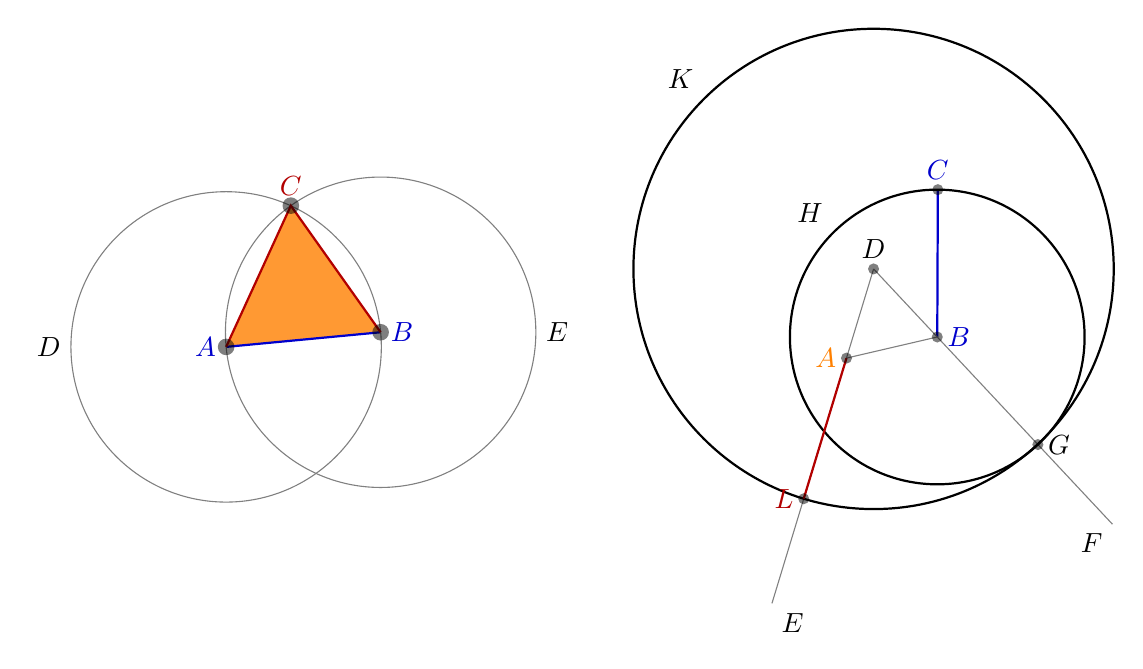
\begin{tikzpicture}[
    thick,help lines/.style={thin,draw=black!50}
  ]
  \begin{scope}[scale=1.5]
    \def\A{\textcolor{input}{$A$}}
    \def\B{\textcolor{input}{$B$}}
    \def\C{\textcolor{output}{$C$}}
    \def\D{$D$} \def\E{$E$}
    \colorlet{input}{blue!80!black}
    \colorlet{output}{red!70!black}
    \colorlet{triangle}{orange}
    \coordinate [label=left:\A] (A) at ($ (0,0) + .1*(rand,rand) $);
    \coordinate [label=right:\B] (B) at ($ (1.25,0.25) + .1*(rand,rand) $);
    \draw [input] (A) -- (B);
    \node [name path=D,help lines,draw,label=left:\D] (D) at (A) [circle through=(B)] {};
    \node [name path=E,help lines,draw,label=right:\E] (E) at (B) [circle through=(A)] {};
    \path [name intersections={of=D and E,by={[label=above:\C]C}}];
    \draw [output] (A) -- (C) -- (B);
    \foreach \point in {A,B,C}
    \fill [black,opacity=.5] (\point) circle (2pt);
    \begin{pgfonlayer}{background}%
      \fill[triangle!80] (A) -- (C) -- (B) -- cycle;
    \end{pgfonlayer}
  \end{scope}
  \begin{scope}[xshift=8cm]
    \def\A{\textcolor{fill}{$A$}}
    \def\B{\textcolor{input}{$B$}}
    \def\C{\textcolor{input}{$C$}}
    \def\D{$D$}\def\E{$E$}\def\F{$F$}
    \def\G{$G$}\def\H{$H$}\def\K{$K$}
    \def\L{\textcolor{output}{$L$}}
    \colorlet{fill}{orange}
    \colorlet{input}{blue!80!black}
    \colorlet{output}{red!70!black}
    \coordinate [label=left:\A] (A) at
    ($(0,0) + .1*(rand,rand) $);
    \coordinate [label=right:\B] (B) at
    ($(1,.2) + .1*(rand,rand) $);
    \coordinate [label=above:\C] (C) at
    ($(1,2) + .1*(rand,rand) $);
    \draw[input] (B)--(C);
    \draw[help lines] (A) -- (B);
    %使用旋转缩放定点法计算点D的坐标
    \coordinate [label=above:\D] (D) at ($(A)!1.0!60:(B)$);
    \draw[help lines] (D) -- ($(D)!3.75!(A)$) coordinate [label=-45:\E] (E);
    \draw[help lines] (D) -- ($(D)!3.75!(B)$) coordinate [label=-135:\F] (F);
    % 半径BC画圆
    \node (H) at (B) [name path = {small circle},circle through = (C),draw,label={135:\H}] {};
    %定位并标记 BF的交点为 G
    \path [name path=BF] (B) -- (F);
    \path [name intersections= {of = BF and {small circle},by={[label=right:\G]G}}];
    %半径DG画圆
    \node (K) at (D) [name path = {big circle},circle through = (G),draw,label={135:\K}] {};
    %定位并标记DE的交点L
    \path [name path=DE] (D) -- (E);
    \path [name intersections={of = DE and {big circle},by={[label=left:\L]L}}];
    \draw[output] (A) -- (L);
    %批量添加阴影
    \foreach \point in {A,B,C,D,L,G}{
        \fill [black,opacity=.5] (\point) circle (2pt);
      }
  \end{scope}
\end{tikzpicture}

\task{Diagrams as Simple Graphs}
\scalebox{.6}{
  \includegraphics{./fig/figure4.png}
}

\step{小彩蛋:设计框线样式\wordbox{nonterminal}与\wordbox{terminal}}
\begin{itemize}
  \item 设置形状参数\wordbox{shape}为\wordbox{rectangle}
  \item 设置尺寸参数\wordbox{minimin size}为\wordbox{6mm}
  \item 设置边框的粗细与颜色参数
  \item 设置边框填充的参数
  \item 设置填充字体的样式
\end{itemize}


\begin{tikzpicture}[
    scale = 2,
    nonterminal/.style={
        rectangle, % shape
        minimum size = 6mm, %size
        very thick, %border
        draw = red!50!black!50,
        top color = white,%the filling
        bottom color = red!50!black!20,
        font=\itshape %font
      }]
  \node [nonterminal] {unsigned integer};% 默认 at (0,0)
\end{tikzpicture}

\vspace{1em}

\begin{tikzpicture}[
    scale = 2,
    node distance=5mm,%设置node之间的距离
    terminal/.style={
        % The shape:
        rectangle,
        minimum size=6mm,
        rounded corners=3mm, % rounded corners
        % The fill
        very thick,
        draw=black!50,
        top color=white,
        bottom color=black!20,
        % The fonts
        font=\ttfamily}]%绘制三个点
  \node (dot) [terminal] {.};
  \node (digit) [terminal,right=of dot] {digit};
  \node (long long digit) [terminal,right=of digit] {long long long long digit};
  \node (E) [terminal,right=of long long digit] {E};
\end{tikzpicture}

\vspace{1em}

\begin{tikzpicture}[
    scale = 2,
    node distance=5mm,%设置node之间的距离
    terminal/.style={
        % The shape:
        rounded rectangle, %shapes.misc提供了等价的rounded rectangle样式
        minimum size=6mm,
        % The fill
        very thick,
        draw=black!50,
        top color=white,
        bottom color=black!20,
        % The fonts
        font=\ttfamily}]%绘制三个点
  \node (dot) [terminal] {.};
  \node (digit) [terminal,right=of dot] {digit};
  \node (long long digit) [terminal,right=of digit] {long long long long digit};
  \node (E) [terminal,right=of long long digit] {E};
\end{tikzpicture}

\step{强迫症狂喜:借助\wordbox{}与\wordbox{}对齐文本\wordbox{baseline}}
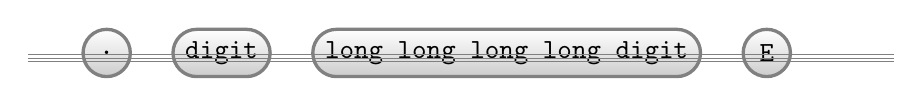
\begin{tikzpicture}[
    scale=2,
    node distance=5mm,
    terminal/.style={
        % The shape:
        rounded rectangle,
        minimum size=6mm,
        % The fill
        very thick,
        draw=black!50,
        top color=white,
        bottom color=black!20,
        % The fonts
        font=\ttfamily}
  ]
  \node (dot) [terminal] {.};
  \node (digit) [terminal,right=of dot] {digit};
  \node (long long digit) [terminal,right=of digit] {long long long long digit};
  \node (E) [terminal,right=of long long digit] {E};
  \draw [help lines]%绘制平行的定位线
  let \p1 = (dot.base),
  \p2 = (digit.base),
  \p3 = (long long digit.base),
  \p4 = (E.base),
  in (-.5,\y1) -- (5.0,\y1)
  (-.5,\y2) -- (5.0,\y2)
  (-.5,\y3) -- (5.0,\y3)
  (-.5,\y4) -- (5.0,\y4);
\end{tikzpicture}

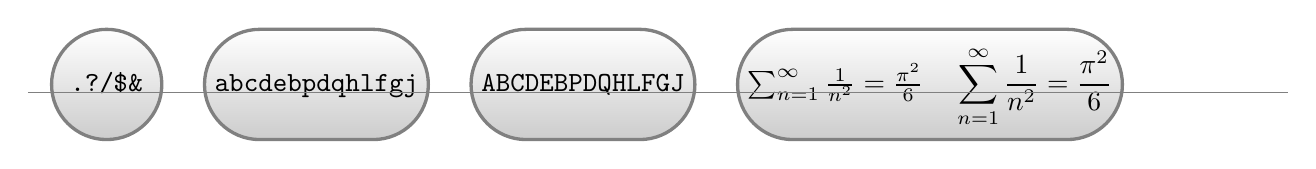
\begin{tikzpicture}[
    scale=2,
    node distance=5mm,
    text height = 1.5ex,%手动设置深度
    text depth = .25ex,
    terminal/.style={
        % The shape:
        rounded rectangle,
        minimum size=14mm,
        % The fill
        very thick,
        draw=black!50,
        top color=white,
        bottom color=black!20,
        % The fonts
        font=\ttfamily}
  ]
  \node (dot) [terminal] {.?/\$\&};
  \node (digit) [terminal,right=of dot] {abcdebpdqhlfgj};
  \node (long long digit) [terminal,right=of digit] {ABCDEBPDQHLFGJ};
  \node (E) [terminal,right=of long long digit] {$\sum_{n=1}^{\infty}\frac{1}{n^2}=\frac{\pi^2}{6}\quad \displaystyle\sum_{n=1}^{\infty}\dfrac{1}{n^2}=\dfrac{\pi^2}{6}$};
  \draw [help lines]%绘制平行的定位线
  let \p1 = (dot.base),
  \p2 = (digit.base),
  \p3 = (long long digit.base),
  \p4 = (E.base),
  in (-.5,\y1) -- (7.5,\y1)
  (-.5,\y2) -- (7.5,\y2)
  (-.5,\y3) -- (7.5,\y3)
  (-.5,\y4) -- (7.5,\y4);
\end{tikzpicture}

\step{基本搭建流程图框架,使用\wordbox{above left}等选项指定斜向相对位置关系}
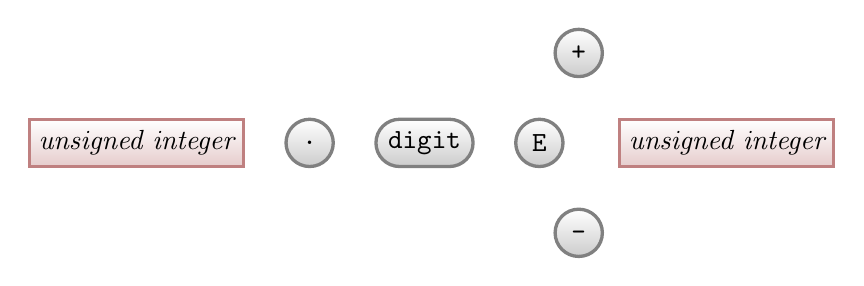
\begin{tikzpicture}[
    scale=2,
    node distance=5mm and 5mm,%使用and同时指定水平&垂直距离
    nonterminal/.style={
        rectangle, % shape
        minimum size = 6mm, %size
        very thick, %border
        draw = red!50!black!50,
        top color = white,%the filling
        bottom color = red!50!black!20,
        font=\itshape %font
      },
    terminal/.style={
        % The shape:
        rounded rectangle,
        minimum size=6mm,
        % The fill
        very thick,
        draw=black!50,
        top color=white,
        bottom color=black!20,
        % The fonts
        font=\ttfamily}
  ]
  \node (ui1) [nonterminal] {unsigned integer};
  \node (dot) [terminal,right=of ui1] {.};
  \node (digit) [terminal,right=of dot] {digit};
  \node (E) [terminal,right=of digit] {E};
  \node (plus) [terminal,above right=of E] {+};
  \node (minus) [terminal,below right=of E] {-};
  \node (ui2) [nonterminal,below right=of plus] {unsigned integer};
\end{tikzpicture}

\tikzset{
  nonterminal/.style={
      rectangle, % shape
      minimum size = 6mm, %size
      very thick, %border
      draw = red!50!black!50,
      top color = white,%the filling
      bottom color = red!50!black!20,
      font=\itshape %font
    },
  terminal/.style={
      % The shape:
      rounded rectangle,
      minimum size=6mm,
      % The fill
      very thick,
      draw=black!50,
      top color=white,
      bottom color=black!20,
      % The fonts
      font=\ttfamily}
}
观察上面的结果我们发现\wordbox{node'+'}和\wordbox{node'-'}的位置由于节点本身的大小限制并不能达到预期,可以尝试采用下面的方式进行修正.
\begin{enumerate}
  \item {
        手动将右侧节点利用\wordbox{xshift}参数进行调整.\par
        \begin{tikzpicture}[node distance=5mm and 5mm]
          \node (E) [terminal] {E};
          \node (plus) [terminal,above right=of E,xshift=5mm] {+};
          \node (minus) [terminal,below right=of E,xshift=5mm] {-};
          \node (ui2) [nonterminal,below right=of plus,xshift=5mm] {unsigned integer};
        \end{tikzpicture}
        }
  \item {利用附加选项参数\wordbox{<style name>/.append style}重新换用\wordbox{rounded corners}参数\par
        \begin{tikzpicture}[node distance=5mm and 5mm,terminal/.append style={rectangle,rounded corners=3mm}]
          \node (E) [terminal] {E};
          \node (plus) [terminal,above right=of E] {+};
          \node (minus) [terminal,below right=of E] {-};
          \node (ui2) [nonterminal,below right=of plus] {unsigned integer};
        \end{tikzpicture}
        }
  \item {使用\wordbox{matrix}更优雅地实现各节点的排布\par
        \begin{tikzpicture}
          \matrix[row sep=1mm,column sep=5mm]{
            %第一行仅在第五个位置为"+"节点
                                                    &   &  &  & \node[terminal]{+};  & \\
            %第二行
            \node[nonterminal] {unsigned interger}; &
            \node[terminal] {.};                    &
            \node[terminal] {digit};                &
            \node[terminal] {E};                    &
                                                    &
            \node[nonterminal] {unsigned interger};                                    \\
            %第三行
                                                    &   &  &  & \node[terminal] {-}; & \\
          };
        \end{tikzpicture}
        }
\end{enumerate}

\step{先来略带痛苦地利用坐标定点绘制出\wordbox{connections}}

\begin{tikzpicture}[scale=1.5,node distance=5mm and 5mm]
  \node (dot) [terminal] {.};
  \node (digit) [terminal,right=of dot] {digit};
  \node (E) [terminal,right=of digit] {E};
  %复习edge的用法
  \path (dot) edge[-latex] (digit) (digit) edge[->] (E);
  \draw [-latex] ($(digit.east)!.5!(E.west)$) -- ++(0,-.5) -| ($(digit.west)!.5!(dot.east)$);
\end{tikzpicture}

但实际上仔细观察发现上面的做法较为麻烦,进一步可以尝试对命令作如下的封装与改进.

\step{为了代码复用,使用\wordbox{to path}选项定义可传入参数的\wordbox{skip loop}样式}
\begin{tikzpicture}[
    scale=1.5,node distance=8mm and 8mm,
    skip loop/.style={to path={-- ++(0,#1) -| (\tikztotarget)}}
  ]% 定义路径,为向y方向shift(#1)单位的距离后垂直延伸 %使用\tikztotarget接受中点参数位置
  \node (dot) [terminal] {.};
  \node (digit) [terminal,right= of dot] {digit};
  \node (E) [terminal,right= of digit] {E};
  \path (dot) edge[-latex] (digit)
  (digit) edge[-latex] (E)
  ($(digit.east)!.5!(E.west)$) edge[-latex,skip loop=-5mm] ($(digit.west)!.5!(dot.east)$);
\end{tikzpicture}

\step{继续折腾更精确的路径节点}
\noindent OS:其实我更建议加入更多参数来调整起始点的精确位置,避免更为复杂的\wordbox{matrix}规划.

\begin{tikzpicture}[
    scale=1.5,node distance=5mm and 5mm,
    point/.style={circle,inner sep=0pt,minimum size=2pt,fill=red},
    skip loop/.style={to path={-- ++(0,#1) -| (\tikztotarget)}}
  ]
  \matrix[row sep=1mm,column sep=2mm] {
    % First row:
                           &                                               &   &  &  &  &  &  &  &  &  & \node (plus) [terminal] {+}; \\
    % Second row:
    \node (p1) [point] {}; & \node (ui1) [nonterminal] {unsigned integer}; &
    \node (p2) [point] {}; & \node (dot) [terminal] {.};                   &
    \node (p3) [point] {}; & \node (digit) [terminal] {digit};             &
    \node (p4) [point] {}; & \node (p5) [point] {};                        &
    \node (p6) [point] {}; & \node (e) [terminal] {E};                     &
    \node (p7) [point] {}; &                                               &
    \node (p8) [point] {}; & \node (ui2) [nonterminal] {unsigned integer}; &
    \node (p9) [point] {}; & \node (p10) [point] {};                                                                                  \\
    % Third row:
                           &                                               &   &  &  &  &  &  &  &  &  & \node (minus)[terminal] {-}; \\
  };
  \path (p4) edge [->,skip loop=-5mm] (p3)
  (p2) edge [->,skip loop=5mm] (p6);
\end{tikzpicture}

\end{document}